\section{Admitere Fb iulie 2023}

2023.A.1. Rezistența echivalentă a două rezistoare conectate în paralel este $2,4 \mathrm{~k} \Omega$. Unul dintre rezistoare are rezistența egală cu $4 k \Omega$. Rezistența celuilalt rezistor este: ( 9 pct.)\\ a) $6000 \Omega$; b) $600 \Omega$; c) $60 \Omega$; d) $60 \mathrm{~k} \Omega$; e) $6 \Omega$; f) $1,6 \mathrm{~k} \Omega$.\\ Rezistența echivalentă a grupării paralel este $R_{e}=\frac{R_{1} R_{2}}{R_{1}+R_{2}} 2$. De unde rezultă: $R_{2}=6 \mathrm{~k} \Omega$. Răspuns corect a.\\

2023.A.2. Un corp cu masa de $2,5 \mathrm{~kg}$ este suspendat de un resort având constanta elastică egală cu $250 \mathrm{~N} / \mathrm{m}$. Alungirea resortului este ($g=10 \mathrm{~m} / \mathrm{s}^{2}$): (9 pct.)\\ a) $10 \mathrm{~cm}$; b) $1 \mathrm{~cm}$; c) $10 \mathrm{~m}$; d) $1 \mathrm{~m}$; e) $4 \mathrm{~cm}$; f) $40 \mathrm{~cm}$.\\ Forța elastică este $F_{e}=k \Delta l$ deci alungirea este $\frac{F}{k}=10 \mathrm{~cm}$. Răspuns corect a.\\

2023.A.3. Un gaz ideal aflat inițial la presiunea de $1 \mathrm{~kPa}$ se destinde izoterm până când volumul său se dublează. Presiunea finală a gazului este: (9 pct.)\\ a) $500 \mathrm{~Pa}$; b) $500 \mathrm{~kPa}$; c) $50 \mathrm{~kPa}$; d) $2 \mathrm{~kPa}$; e) $1 \mathrm{~Pa}$; f) $4 \mathrm{~kPa}$.\\ Din legea transformării izoterme rezultă $P_{2}=\frac{P_{1} V_{1}}{V_{2}}=500 \mathrm{~Pa}$. Răspuns corect a.\\

2023.A.4. Un motor funcționează după un ciclu Carnot între două rezervoare termice având temperaturile de $900 \mathrm{~K}$ şi $300 \mathrm{~K}$. În fiecare ciclu, motorul efectuează un lucru mecanic de $1200 \mathrm{~J}$. Căldura cedată sursei reci într-un ciclu este: (9 pct.)\\ a) $600 \mathrm{~J}$; b) $1800 \mathrm{~J}$; c) $660 \mathrm{~J}$; d) $1320 \mathrm{~J}$; e) $400 \mathrm{~J}$; f) $2400 \mathrm{~J}$.\\ Randamentul unui motor termic este $\eta=\frac{L}{Q_{\text {prim}}}$. Din conservarea energiei, $Q_{\text {prim}}=L+ \left|Q_{ced}\right|$. Randamentul ciclului Carnot este $\eta=1-\frac{T_{2}}{T_{1}}$, de unde rezultă $\left|Q_{ced}\right|=\frac{T_{2} L}{T_{1}-T_{2}}=600 \mathrm{~J}$. Răspuns corect a.\\

2023.A.5. Un circuit este format dintr-o sursă cu t.e.m. de $12 \mathrm{~V}$ și rezistența internă de $6 \Omega$ şi un rezistor cu rezistență variabilă. Puterea maximă ce poate fi debitată în rezistor este: (9 pct.)\\ a) $6 \mathrm{~W}$; b) $2 \mathrm{~W}$; c) $24 \mathrm{~W}$; d) $12 \mathrm{~W}$; e) $72 \mathrm{~W}$; f) $1 \mathrm{~W}$.\\ Puterea maximă debitată într-un circuit se obține când rezistența circuitului este egală cu rezistența internă a sursei: $P=I^{2} r=\frac{E^{2}}{4 r}=6 \mathrm{~W}$. Răspuns corect a.\\

2023.A.6. Legea de mişcare a unui punct material cu masa de $2 \mathrm{~kg}$ este $x(t)=5+6t+1,5t^{2}$, unde $x$ este măsurat în metri, iar $t$ în secunde. Forța care acționează asupra punctului material este: (9 pct.)\\ a) $6 \mathrm{~N}$; b) $3 \mathrm{~N}$; c) $16 \mathrm{~N}$; d) $1,5 \mathrm{~N}$; e) $12 \mathrm{~N}$; f) $10 \mathrm{~N}$.\\ Din legea mişcării rezultă: $\frac{a}{2}=1,5 \mathrm{~m} / \mathrm{s}^{2}$, de unde $a=3 \mathrm{~m} / \mathrm{s}^{2}$.\\ Deci forța care acționează este $F=m a=6 \mathrm{~N}$. Răspuns corect a.\\

2023.A.7. Un circuit electric este format din trei surse ideale de tensiune cu t.e.m. de $100 \mathrm{~V}$, patru rezistoare, fiecare având rezistența $R$ de $4 \Omega$ şi un rezistor cu rezistența variabilă $R_{x}$, conectate ca în figură. Dacă tensiunea la bornele rezistorului $R_{x}$ este de $34 \mathrm{~V}$, intensitatea curentului prin acesta are valoarea: ( 9 pct.)\\ a) $4 \mathrm{~A}$; b) $5 \mathrm{~A}$; c) $6 \mathrm{~A}$; d) $7 \mathrm{~A}$; e) $8 \mathrm{~A}$; f) $9 \mathrm{~A}$.\\ 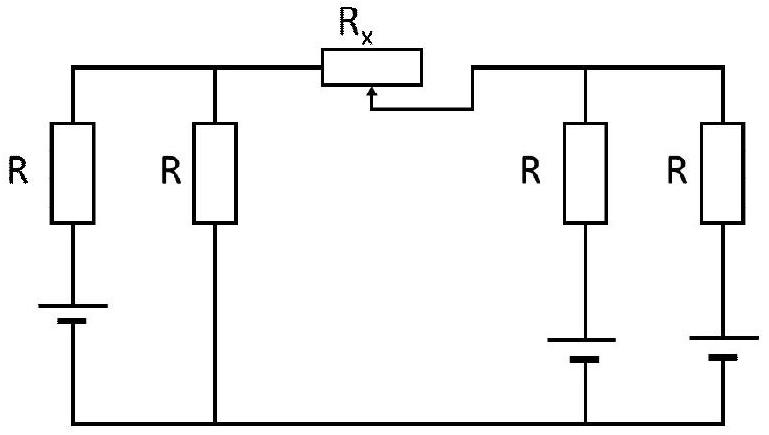
\includegraphics[width=0.4\linewidth]{images/2025_08_19_17c3b9471cd89f0defc4g-02(1)}\\ Circuitul poate fi simplificat considerând o grupare paralel a două surse de tensiune electromotoare $E$ și rezistența internă $R$. Astfel, se obține schema echivalentă din figură în care se aplică legea lui Kirchoff:\\ \begin{center} 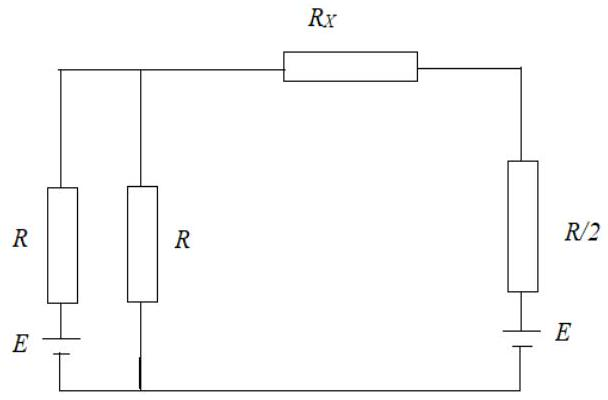
\includegraphics[width=0.4\linewidth]{images/2025_08_19_17c3b9471cd89f0defc4g-03(1)} \end{center}\\ $\left\{\begin{array}{c} 2 I_{1} R+I R=E \\ I \frac{R}{2}+I R_{x}+I_{1} R+I R=E \end{array}\right.$, unde $I R_{x}=U$\\ De aici rezultă: $I=\frac{E-2 U}{2 R}=4 \mathrm{~A}$. Răspuns corect a.\\

2023.A.8. Un corp cu masa de $1000 \mathrm{~g}$ este lansat de la baza unui plan înclinat, în lungul acestuia, cu viteza de $4 \mathrm{~m} / \mathrm{s}$. Corpul revine la baza planului înclinat cu o viteză egală cu jumătate din viteza inițială. Lucrul mecanic al forțelor de frecare dintre corp şi plan este: (9 pct.)\\ a) $-6 \mathrm{~J}$; b) $-3 \mathrm{~J}$; c) $-1 \mathrm{~J}$; d) $-12 \mathrm{~J}$; e) $-18 \mathrm{~J}$; f) $-5 \mathrm{~J}$.\\ Din teorema de variație a energiei cinetice rezultă $\left|L_{Ff}\right|=\left|\frac{m v^{2}}{2}-\frac{m v_{0}^{2}}{2}\right|=6 \mathrm{~J}$. Răspuns corect a.\\

2023.A.9. În cursul unui proces izobar, lucrul mecanic efectuat de un gaz ideal reprezintă un sfert din căldura primită. Exponentul adiabatic al gazului este: (9 pct.)\\ a) $\frac{4}{3}$; b) $\frac{7}{5}$; c) $\frac{8}{5}$; d) $\frac{10}{7}$; e) $\frac{3}{2}$; f) $\frac{5}{3}$.\\ Folosim relația dintre căldură și lucru mecanic:\\ $L=\frac{1}{4} Q \Rightarrow \nu R \Delta T=\frac{1}{4} \nu C_{p} \Delta T \Rightarrow C_{p}=4 R$;\\ Conform relației Rober-Mayer, $C_{p}-C_{V}=R \Rightarrow C_{V}=C_{p}-R=4 R-R=3 R$.\\ Obținem exponenul adiabatic $\gamma=\frac{C_{p}}{C_{V}}=\frac{4 R}{3 R}=\frac{4}{3}$. Răspuns corect a.\\ 

2023.A.10. Viteza unui mobil aflat în mişcare rectilinie este reprezentată în figură. Viteza medie a mobilului în intervalul de timp cuprins între $t_{1}=1 \mathrm{~s}$ şi $t_{2}=5 \mathrm{~s}$ este: (9 pct.)\\ a) $3,75 \mathrm{~m} / \mathrm{s}$; b) $5 \mathrm{~m} / \mathrm{s}$; c) $10 \mathrm{~m} / \mathrm{s}$; d) $7,5 \mathrm{~m} / \mathrm{s}$; e) $11,25 \mathrm{~m} / \mathrm{s}$; f) $4,5 \mathrm{~m} / \mathrm{s}$.\\ 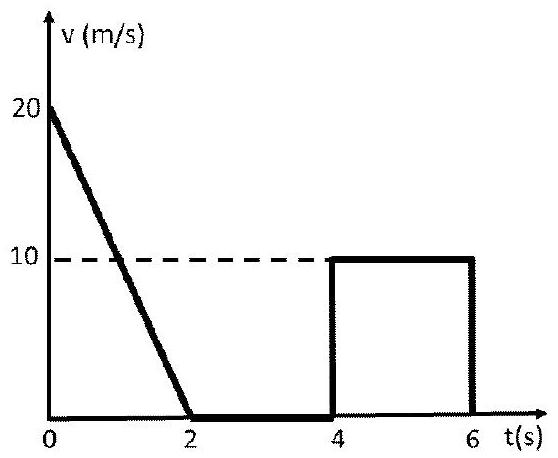
\includegraphics[width=0.4\linewidth]{images/2025_08_19_17c3b9471cd89f0defc4g-02}\\ Graficul este format din 3 zone în intervalul $t_{1}=1 \mathrm{~s}$ și $t_{2}=5 \mathrm{~s}$:\\ Între $t=1 \mathrm{~s}$ și $t=2 \mathrm{~s}$, este o dreaptă descendentă de la $10 \mathrm{~m} / \mathrm{s}$ la $0 \mathrm{~m} / \mathrm{s}$, deci aflăm distanța din aria triunghiului: $d_{1}=\frac{1}{2}(2-1)(10-0)=5 \mathrm{~m}$.\\ Între $t=2 \mathrm{~s}$ și $t=4 \mathrm{~s}$, viteza este nulă, deci $d_{2}=0 \mathrm{~m}$.\\ Între $t=4 \mathrm{~s}$ și $t=5 \mathrm{~s}$, viteza este constantă, deplasarea aflându-se din aria dreptunghiului: $d_{3}=(5-4) \cdot 10=10 \mathrm{~m}$.\\ Din toate, deplasarea totală este $\Delta d=d_{1}+d_{2}+d_{3}=15 \mathrm{~m}$.\\ Deci viteza medie este: $v_{m}=\frac{\Delta d}{\Delta t}=\frac{15}{4}=3,75 \mathrm{~m} / \mathrm{s}$. Răspuns corect a.\\
